\documentclass[12pt]{article} % use larger type; default would be 10pt
\usepackage[utf8]{inputenc} % set input encoding (not needed with XeLaTeX)

%%% PAGE DIMENSIONS
\usepackage{geometry} % to change the page dimensions
\geometry{a4paper} % or letterpaper (US) or a5paper or....
\geometry{margin=2cm} % or letterpaper (US) or a5paper or....

\usepackage{graphicx} % support the \includegraphics command and options
\usepackage[parfill]{parskip} % Activate to begin paragraphs with an empty line rather than an indent
\usepackage{times} % for Times Roman default font

%%% PACKAGES
\usepackage{booktabs} % for much better looking tables
\usepackage{array} % for better arrays (eg matrices) in maths
\usepackage{paralist} % very flexible & customisable lists (eg. enumerate/itemize, etc.)
\usepackage{verbatim} % adds environment for commenting out blocks of text & for better verbatim
\usepackage{subfig} % make it possible to include more than one captioned figure/table in a single float

%%% HEADERS & FOOTERS
\usepackage{fancyhdr} % This should be set AFTER setting up the page geometry
\pagestyle{fancy} % options: empty , plain , fancy
\renewcommand{\headrulewidth}{0pt} % customise the layout...
\lhead{}\chead{}\rhead{}
\lfoot{}\cfoot{\thepage}\rfoot{}

\makeatletter
\renewcommand{\maketitle}{%
  \begin{center}
    {\bfseries{\scshape{\Large{\@title\par}}}}
  \end{center}
  \medskip
  \begin{flushright}
    {\@date\par}
  \end{flushright}
    \bigskip\hrule\vspace*{2pc}%
}
\makeatother

\hyphenation{Kiwi-bank} % otherwise it may get hyphenated as Ki-wibank

%%% END Article customizations

%%% The "real" document content comes below...

\title{Springs Tramping Base}
%\author{}
\date{\today} % Activate to display a given date or no date (if empty),
         % otherwise the current date is printed 

\begin{document}
  \maketitle

\begin{figure}[t]
%\centering
\begin{minipage}{.3\linewidth}
\begin{flushleft} 
   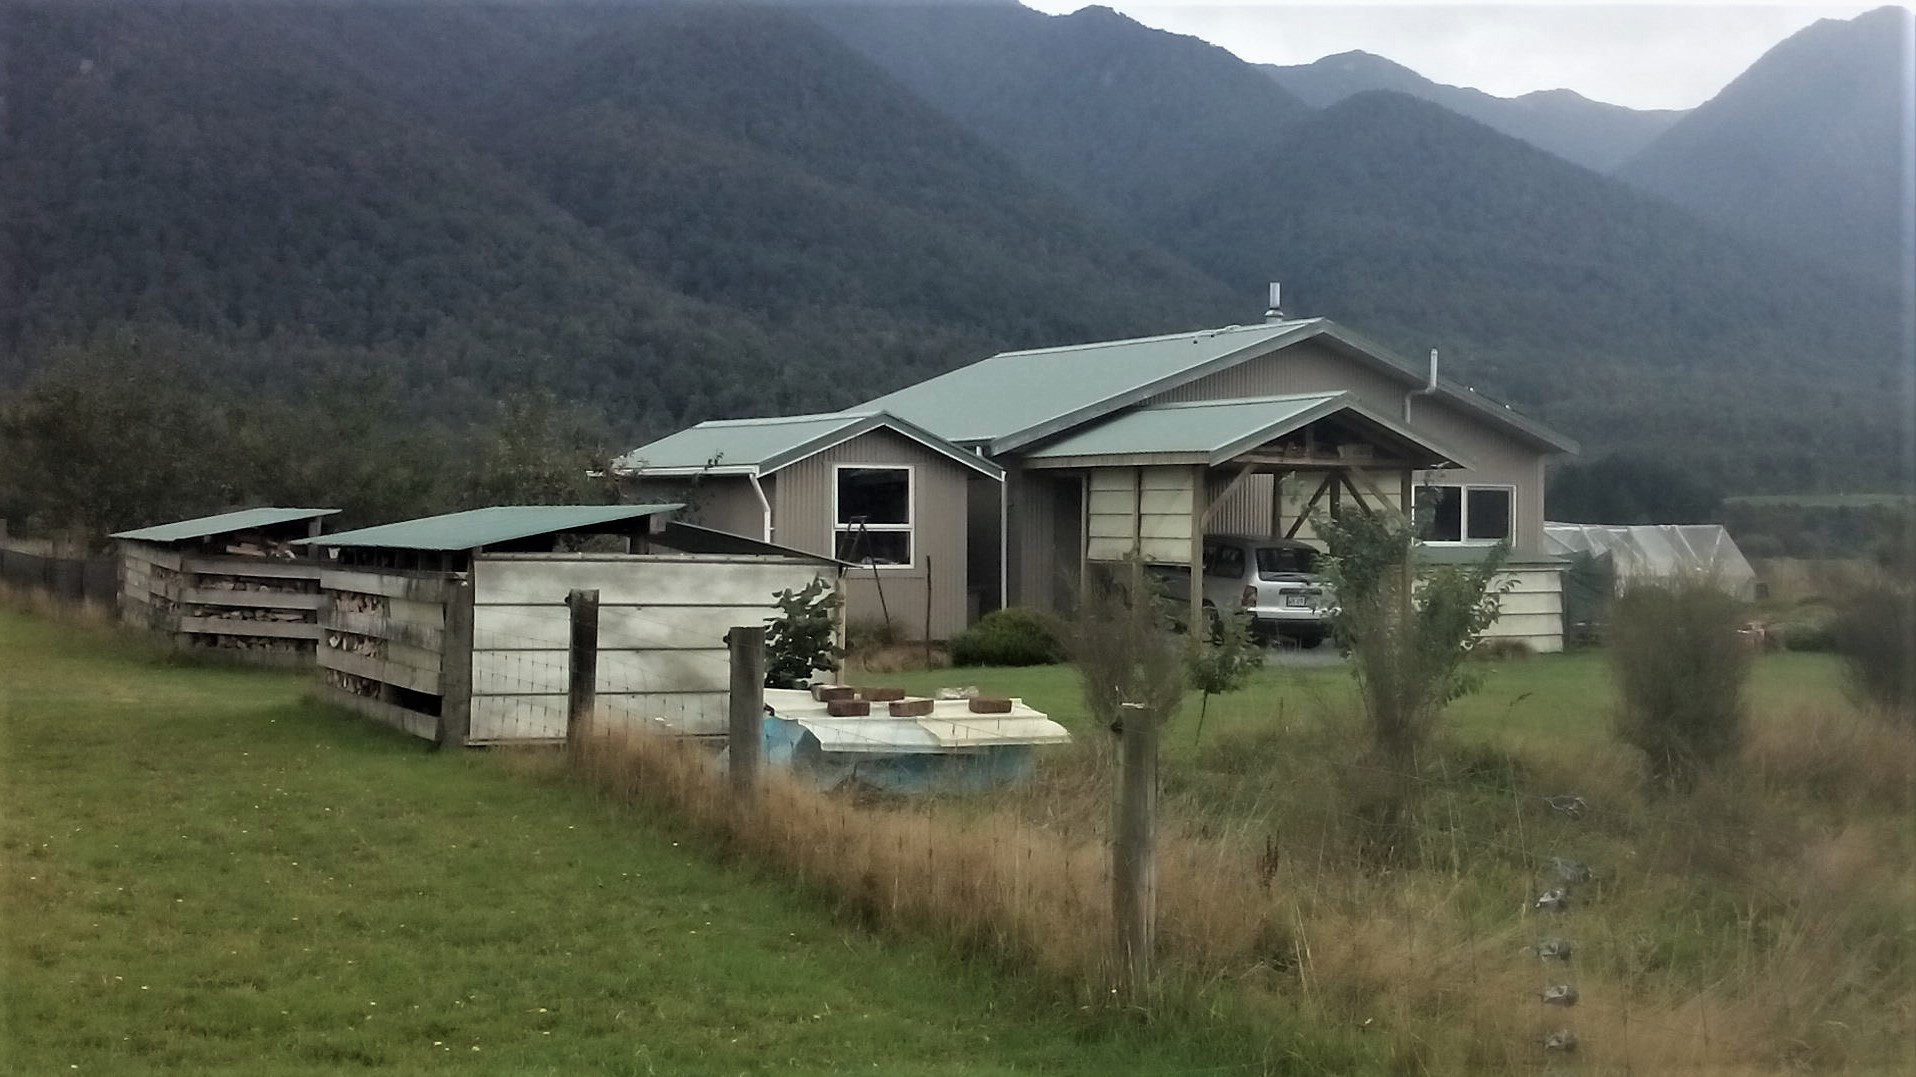
\includegraphics[width=4.5cm]{BachPhoto}
\end{flushleft} 
\end{minipage}
\begin{minipage}{.3\linewidth}
\begin{center} 
   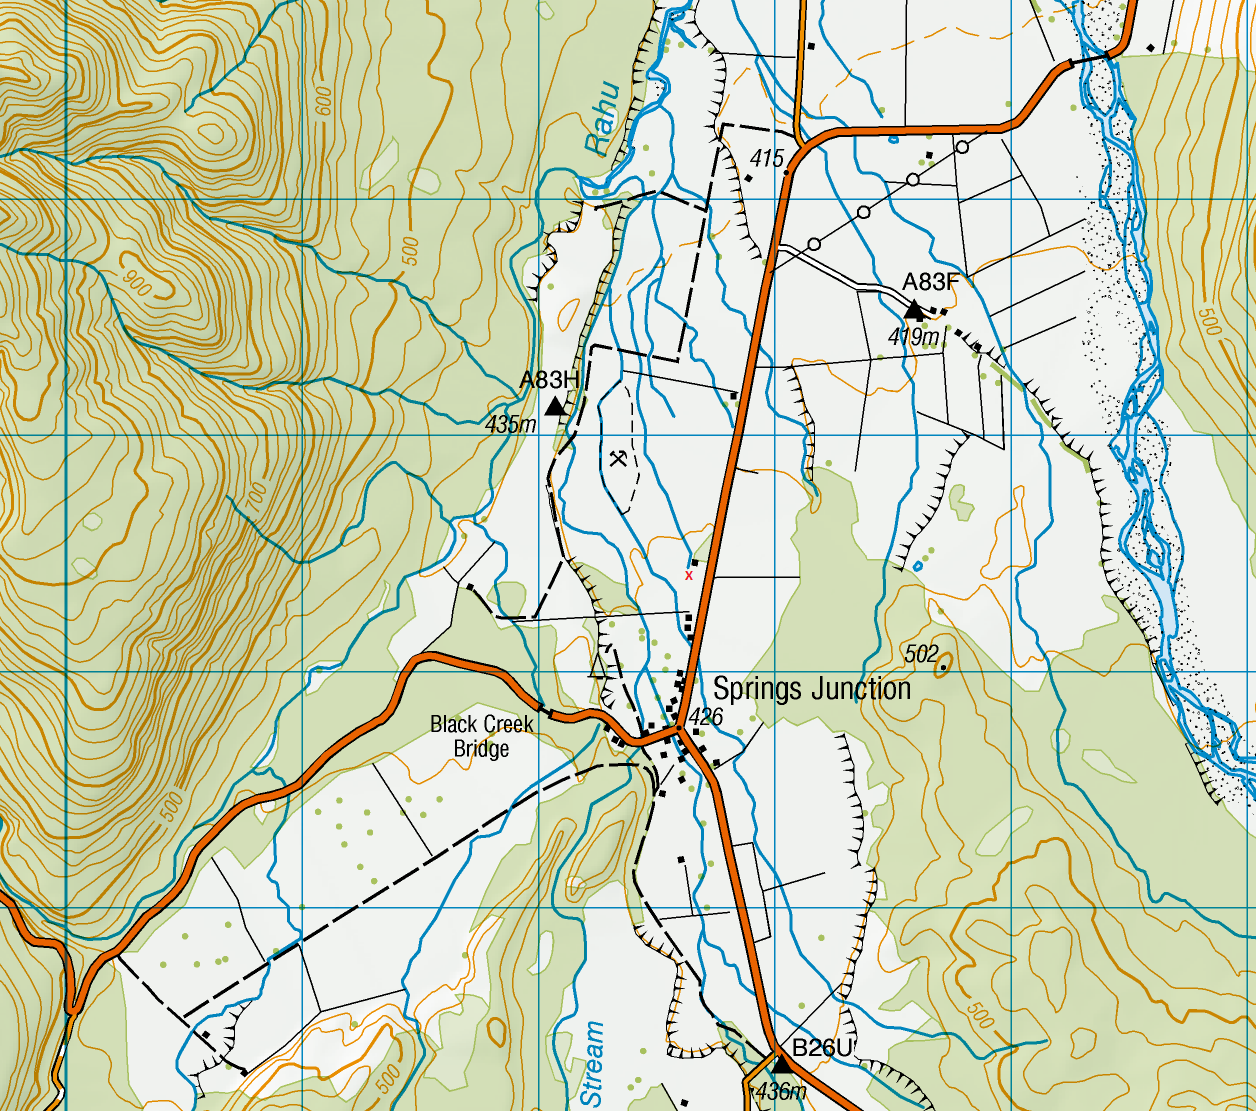
\includegraphics[width=5.5cm]{BachLocation}
\end{center} 
\end{minipage}
\hspace{.05\linewidth}
\begin{minipage}{.3\linewidth}
\begin{flushright} 
    \includegraphics[width=4.5cm]{BachInSnow}
\end{flushright} 
\end{minipage}
\end{figure}

  \section{Directions}
    The house is on the west side of Highway 65 at the 60kph sign just
    to the north of Springs Junction.  It is through the second gate on the
    right off ``Josie's Way''.  Currently it is the only building on
    the sub-division.

  \section{Keys}
  \begin{itemize}
    \item The key to the gate (``Josie's Way'') is at the hinge end under
    the top rail.
    \item The key to the house is in the secure key lock on the wood shed (combination 1427).  It opens the west door.  Note,
    door handle must be horizontal to open.  This applies to all external doors and windows, and they all open inward.
  \end{itemize}

  \section{Your stay}
  \begin{itemize}
    \item You are welcome to use any items, but next time you come
    please replace consumables with the equivalent item.  Try not to
    use the last of any consumable if you are unable to replace it
    before you leave.
    \item Please turn the gas to the stove off outside when
      you have finish cooking.
    \item The 10l white food-grade plastic bucket (with lid) is for
      drinking water only.
    \item The deep hole on the west side is a ``poor person's cellar''
      for keeping perishables cool.
    \item The water in the taps comes from the bore and may taste of iron for a while; that from the tank is rain-water.  Neither have been tested.
    \item If you need to access the pump, the combination lock opens after 3 turns clockwise stop at 3, turn anti-clockwise passed 3 and stop at 26, turn clock-wise to stop at 20 and release lock.
    \item I am vegetarian and prefer that meat is not fried inside.
    \item The `Pyroclassic' fire came with detailed instructions.  If you
      are having trouble with it, then please read these.  In a
      peculiar way, they are entertaining.  It is best to allow it to build up a good bed of embers before closing the bottom vent.
    \item There is a heat-exchanger in the fire which heats the hot water.  In teh summer, the solar panels generally do the job.
    \item The outdoor bath takes 1-1.5 hours to heat (if the cover
      is put on it).  There is a blue pseudo-sheepskin mat hanging up by the `Pyroclassic' fire to sit on when in the bath (the base of the bath can get quite hot).
    \item \textbf{No smoking} in the bach or on the decking.  If
    smoking outside, please do not litter (i.e., take the butts home).
    \item Please take all non-compostable rubbish home.
    \item Please report any damage to me as soon as possible.
    \item Please fill-in the Visitor's Book, and note any interesting
      trips in the Journal.
    \item The house is off-grid (i.e., power entirely from the solar panels).  The system is deliberately marginal so that one has to be conscious of power usage.  The inverter is pure sine-wave and should be safe for electronic equipment.
  \end{itemize}
 
  \subsection{Toilet}
    The Kiwi-bog is an exclusively sit-down facility (men may pee outside on the plants).  There are instructions on the shelf in the toilet: \textbf{please read these}.  Urine flows into a bucket located under a plywood cover outside the toilet window.  The urine should be diluted and used to fertigate the plants when you leave.  Cover faeces with a
    small amount of wood shavings (less than the volume of faeces).  When the bucket is
    about two-thirds full it should be emptied in the black plastic compost bin
    outside.  Cover with an arm-full of grass.  Wash the bucket and
    return to the toilet.  Cover the bottom of the bucket with a
    layer of wood shavings.

    Compostable vegetable material can be put into the wooden compost bin by the bath.  Please don't put meat scraps in either the toilet or compost bin
    (bury them or take them home).

  \subsection{Hazards}
    Care should be taken with the ladder to the sleeping
    loft (it is a ladder not stairs).

  \section{On leaving}
  \begin{itemize}
    \item Ensure all doors and windows are closed and locked (\textbf{handle pointing down}).
    \item Check that the gas cylinder to the stove is off.
    \item Empty the urine bucket (see above).
    \item Please leave the place clean and tidy - endeavour to leave
    it a bit cleaner and tidier than you found it.
    \item Lock the west door and return the key to the secure key lock.
    \item Close all gates, and lock the main gate (and ensure the key
      is in its correct place on the nail).
  \end{itemize}


\bigskip
Peter Alspach\\paalspach@gmail.com\\(022) 528 7529

\end{document}
